\section{Part 1}
\subsection{Assignment 3 - myon energy loss}

\begin{table}
\centering
\caption{Myon momentum in inner and outer detector}
\begin{tabular}{ccc}
\toprule
n & $p_{in}/\si{GeV}$ & $p_{out}/\si{GeV}$\\
\midrule
1 & / & /\\
2&	-85&	-53.92\\
3&	43.4&	43.83\\
4&	-241.37&	-237.02\\
5&	48.89&	44.77\\
6&	-168.16&	-177.62\\
7&	117.32&	96.56\\
8&	-71.94&	-64.96\\
9&	199.91&	199.44\\
10&	-57.84&	-50.01\\
11&	/ & /\\
12&-100.75&	-94.11\\
13&	38.26&	34.48\\
14&	-105.19&	-108.68\\
15&	236.12&	236.61\\
16&	-131.69&	-125.51\\
17&	152.24&	157.69\\
18&	-35.23&	-32.18\\
19&	54.19&	50\\
20&	-84.75&	-68.09\\
21&	104.26&	107.98\\
22&	-184.01&	-170.66\\
23&	100.36&	101.13\\
\bottomrule
\end{tabular}
\label{tab:task1_myon}
\end{table}

In tabular \ref{tab:task1_myon} the measured momentum in the inner and outer detector part are given for the first 23 events. In event 1 and 11 the myon trace did not continue to the outer part. The energy loss is now given by $\Delta E = |p_out| - |p_in|$ (note that the myons can be treated like relativistic particles). The mean energy loss is given by $\Delta E = \si{5 \pm 9\,GeV}$.

\subsection{Assignment 6 - $Z_0 \to e^+ e^-$ invariant mass}
\begin{table}
\centering
\caption{Electron/positron momentum and the invariant mass $m$}
\begin{tabular}{ccccc}
\toprule
n & $p_1$/GeV & $p_2$/GeV & $m_1$/GeV & $m_2$/GeV\\
\midrule
1 &	-115.81&	63.29 & 171.23 & 171.23\\ 
2&	-49.69&	60.92 & 110.04 & 110.04\\
3&	-78.58&	101.01& 178.18 & 178.18\\
\bottomrule
\end{tabular}
\label{tab:task1_zee}
\end{table}

In tabular \ref{tab:task1_zee} the momentum of the $e^+/e^-$ is given together with the corresponding invariant mass. The invariant mass was calculated in two ways, first using the electron mass and second neglecting the electron mass. As one can see the electron mass does not have an influence on the invariant mass (So the electrons can be treated as ultra relativistic). 

\section{Part 2}
\begin{figure}
\centering
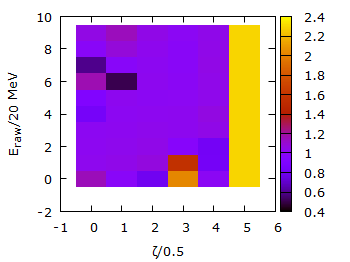
\includegraphics[scale=1]{data/zee_init/zee_init.png}
\caption{Correction factor $E_e/E_{\mathrm{raw}}$ over $E_{\mathrm{raw}}$ and $\eta$}
\label{fig:part2_factor}
\end{figure}

In figure \ref{fig:part2_factor} the correction factor $E_e/E_{\mathrm{raw}}$ is plotted over the raw energy $E_{\mathrm{raw}}$ and $\eta$. 

\section{Part 3 - W Boson mass}

The QCD scale factor was set to $0.33$.

\begin{table}
\centering
\caption{Measured half maxima $h$ for different W boson masses}
\begin{tabular}{ccccc}
\toprule
$m_W$/MeV & $h$/Gev & $\Delta h$/GeV\\ 
\midrule
75&	40.18&	0.06\\
78&	41.78&	0.07\\
79&	42.25&	0.06\\
80&	42.85&	0.06\\
81&	43.46&	0.07\\
82&	43.79&	0.07\\
85&	45.49&	0.11\\
\bottomrule
\end{tabular}
\label{tab:task3_33}
\end{table}